\newpage
\subsection{Mean and standard error}

\begin{figure}[!h]
    \centering
    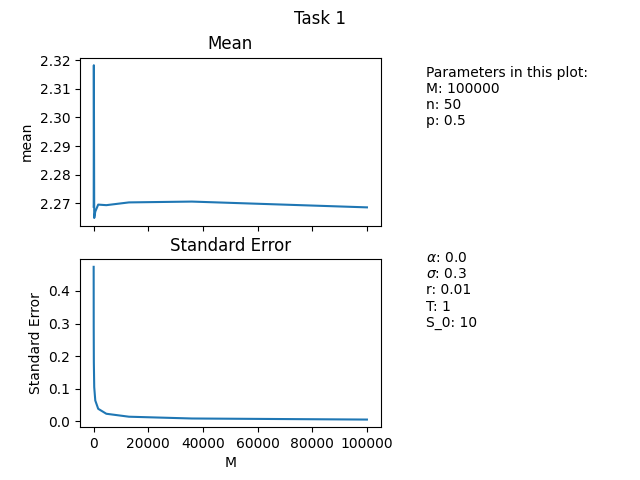
\includegraphics[width=0.7\linewidth]{pictures/task1.png}
    \caption{Dependency on M}
    \label{fig:task1}
\end{figure}


\newpage
\subsection{Sensitivity analysis of floating strike lookback put and comparison to European Put}

\subsubsection{Note towards pikes in the graphs}
\begin{figure}[!h]
    \centering
    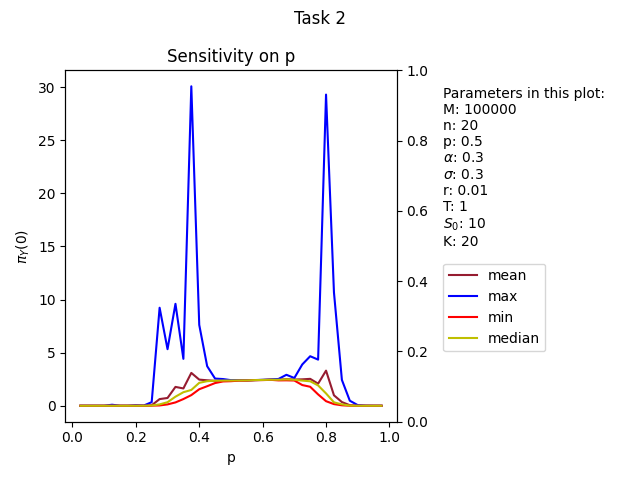
\includegraphics[width=0.7\linewidth]{pictures/spike_evaluation.png}
    \caption{Dependency on M}
    \label{fig:spike}
\end{figure}

There are very dominant spikes in the curve and to find out what causes them I created this plot, which compares different measures of the data set. As it can be seen there are some extreme outliers which cause the mean to spike. This suggests that maybe the median would be a better measure, but this would require some further investigation.

\newpage
\subsubsection{Probability p}
\begin{figure}[!h]
    \centering
    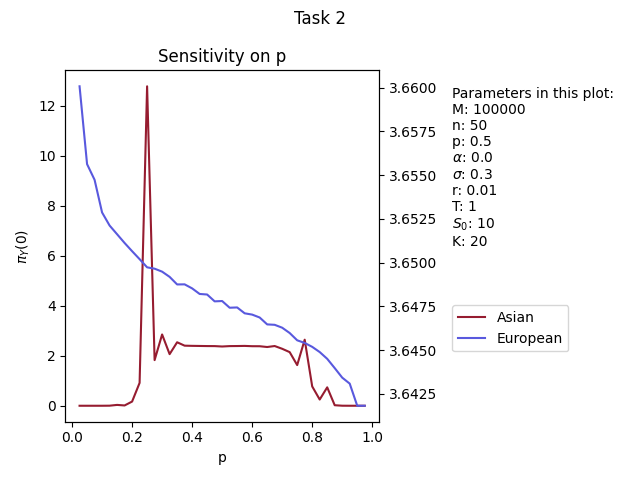
\includegraphics[width=0.7\linewidth]{pictures/task2_p.png}
    \caption{Dependency on p}
    \label{fig:task2_p}
\end{figure}

On the edges the initial value of the derivative is basically zero. As those values basically suggest that the outcome is almost predictable, this is not surprising as there would be better options available for the investor. For example if it is known that p is very close to 1 (~0.9) than the investor would be better off buying the stock instead. As it will be very likely that the maximum appears very close towards maturity and thus must be very close to the strike price this results in a minimal payoff.
Similar reasoning goes for very low chances of increasing stock prices, here the initial stock price will likely be the maximum or be close to the maximum and therefore the payoff is caped by the initial price.
I would have expected that the rise in the beginning is slower than the fall off at the end. This might be the case as the stock grows exponentially, so in the end the price is very high. If now in the last few steps a decline occurs, it will be quite significant and thus result in a relatively high payoff. This seems however not to be the case. But this might be counteracted by the lower probability of this happening.

In the center there is a relatively flat plane … why? Also why is is symmetric? 

Although the European seems to be related to p, looking at the y-scaling reveals that this is  neglectably small.

Add Chengji formula approach

\newpage
\subsubsection{Mean of log return $\alpha$}
\begin{figure}[!h]
    \centering
    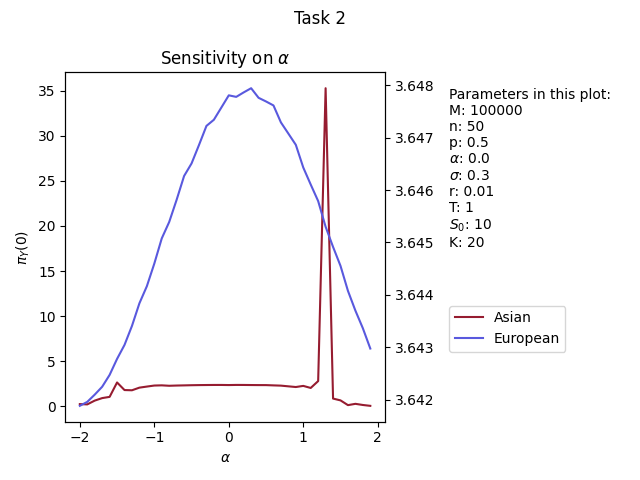
\includegraphics[width=0.7\linewidth]{pictures/task2_alpha.png}
    \caption{Dependency on $\alpha$}
    \label{fig:task2_alpha}
\end{figure}

With negative alpha both up and down movements are decreasing the stock price value (given sufficiently low volatility). This would mean for negative alpha the payoff should converge towards S0 and thus generate a capped, but somewhat predictable profit. 

If on the other hand alpha gets larger I would expect the price of the put option to fall as it gets more likely that the maximum occurs towards the end.

The maximum appears at 0.0, given a p of 0.5, the process should be a martingale here and thus larger payoffs are only steered by volatility. 

\newpage
\subsubsection{Volatility $\sigma$}
\begin{figure}[!h]
    \centering
    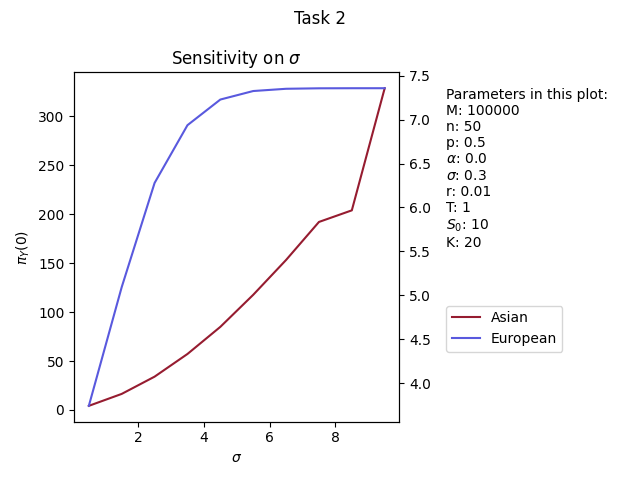
\includegraphics[width=0.7\linewidth]{pictures/task2_sigma.png}
    \caption{Dependency on $\sigma$}
    \label{fig:task2_sigma}
\end{figure}

With rising volatility the initial price of the option increases. As both the increases and decreases of the stock price become more distinctive. With low volatility the spread is 

Generally I think such a smooth relation is surprising as with growing volatility the outcome becomes more unpredictable. This would however be aline with the general principle of “higher risk higher profit”.

There could be very a beneficial drop in the price. As there is no tendency towards upwards or downwards movement, those fluctuations could appear in any direction, however there exists no upper limit but a lower one at 0. Thus, those two don’t counteract.


The European behave just as in the lecture notes, to it reaches some maximum at some point.

\newpage
\subsubsection{Risk free rate r}
\begin{figure}[!h]
    \centering
    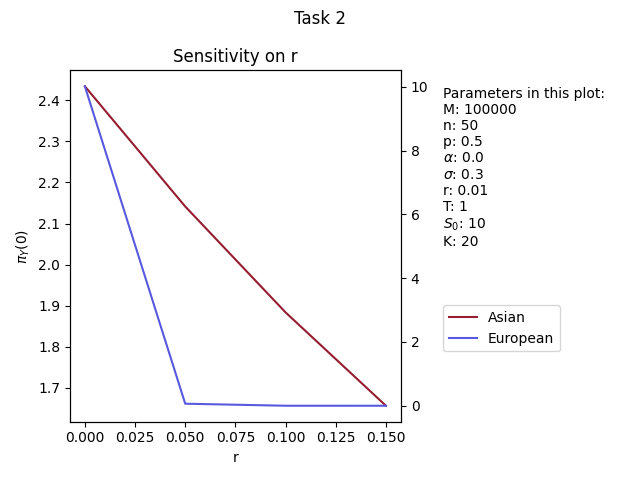
\includegraphics[width=0.7\linewidth]{pictures/task2_r.png}
    \caption{Dependency on r}
    \label{fig:task2_r}
\end{figure}


This relation seems to be what is expected. If r grows it becomes more and more attractive for investors to buy risk free assets instead and thus the price of the put must plummet.

The European put behaves in a similar way, but it declines faster until it reaches zero. This is however a function of K, so generally both options are very similar in their relation to changing r.

\newpage
\subsubsection{Maturity date T}
\begin{figure}[!h]
    \centering
    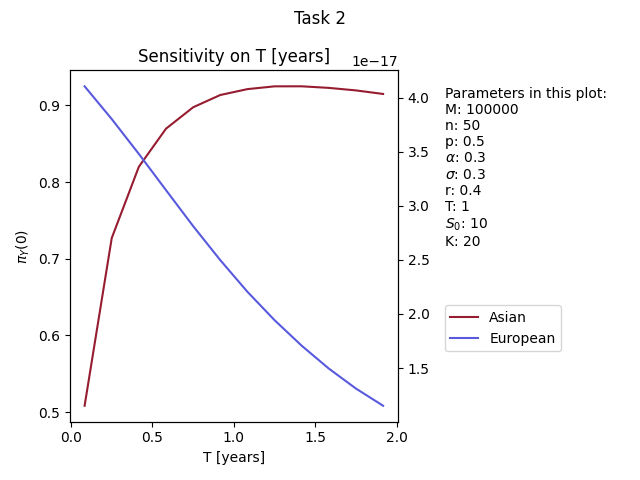
\includegraphics[width=0.7\linewidth]{pictures/task2_T.png}
    \caption{Dependency on T}
    \label{fig:task2_T}
\end{figure}


The longer the investors have to wait the higher is the value in the beginning.
Interestingly, the European option seems to be following the exact opposite path, but actually the relation is minimal as the absolute value of the initial put price doesn’t significantly change.

If longer time spans or higher risk free rates are investigated the initial value of the Asian put will decline as well, as it becomes more attractive to buy a risk free asset instead.

\newpage
\subsubsection{Initial stock price $S_0$}
\begin{figure}[!h]
    \centering
    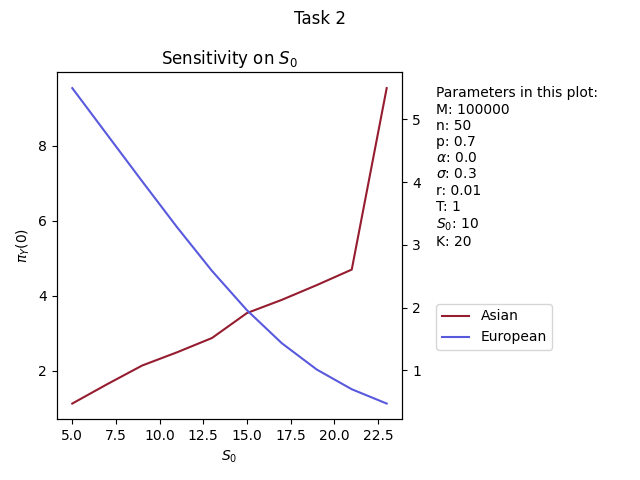
\includegraphics[width=0.7\linewidth]{pictures/task2_S_0.png}
    \caption{Dependency on $S_0$}
    \label{fig:task2_S_0}
\end{figure}

Europ: Take Chengji
Asian: Differences will be greater